\documentclass[a4paper]{article}\usepackage{graphicx, color}
%% maxwidth is the original width if it is less than linewidth
%% otherwise use linewidth (to make sure the graphics do not exceed the margin)
\makeatletter
\def\maxwidth{ %
  \ifdim\Gin@nat@width>\linewidth
    \linewidth
  \else
    \Gin@nat@width
  \fi
}
\makeatother

\IfFileExists{upquote.sty}{\usepackage{upquote}}{}
\definecolor{fgcolor}{rgb}{0.2, 0.2, 0.2}
\newcommand{\hlnumber}[1]{\textcolor[rgb]{0,0,0}{#1}}%
\newcommand{\hlfunctioncall}[1]{\textcolor[rgb]{0.501960784313725,0,0.329411764705882}{\textbf{#1}}}%
\newcommand{\hlstring}[1]{\textcolor[rgb]{0.6,0.6,1}{#1}}%
\newcommand{\hlkeyword}[1]{\textcolor[rgb]{0,0,0}{\textbf{#1}}}%
\newcommand{\hlargument}[1]{\textcolor[rgb]{0.690196078431373,0.250980392156863,0.0196078431372549}{#1}}%
\newcommand{\hlcomment}[1]{\textcolor[rgb]{0.180392156862745,0.6,0.341176470588235}{#1}}%
\newcommand{\hlroxygencomment}[1]{\textcolor[rgb]{0.43921568627451,0.47843137254902,0.701960784313725}{#1}}%
\newcommand{\hlformalargs}[1]{\textcolor[rgb]{0.690196078431373,0.250980392156863,0.0196078431372549}{#1}}%
\newcommand{\hleqformalargs}[1]{\textcolor[rgb]{0.690196078431373,0.250980392156863,0.0196078431372549}{#1}}%
\newcommand{\hlassignement}[1]{\textcolor[rgb]{0,0,0}{\textbf{#1}}}%
\newcommand{\hlpackage}[1]{\textcolor[rgb]{0.588235294117647,0.709803921568627,0.145098039215686}{#1}}%
\newcommand{\hlslot}[1]{\textit{#1}}%
\newcommand{\hlsymbol}[1]{\textcolor[rgb]{0,0,0}{#1}}%
\newcommand{\hlprompt}[1]{\textcolor[rgb]{0.2,0.2,0.2}{#1}}%

\usepackage{framed}
\makeatletter
\newenvironment{kframe}{%
 \def\at@end@of@kframe{}%
 \ifinner\ifhmode%
  \def\at@end@of@kframe{\end{minipage}}%
  \begin{minipage}{\columnwidth}%
 \fi\fi%
 \def\FrameCommand##1{\hskip\@totalleftmargin \hskip-\fboxsep
 \colorbox{shadecolor}{##1}\hskip-\fboxsep
     % There is no \\@totalrightmargin, so:
     \hskip-\linewidth \hskip-\@totalleftmargin \hskip\columnwidth}%
 \MakeFramed {\advance\hsize-\width
   \@totalleftmargin\z@ \linewidth\hsize
   \@setminipage}}%
 {\par\unskip\endMakeFramed%
 \at@end@of@kframe}
\makeatother

\definecolor{shadecolor}{rgb}{.97, .97, .97}
\definecolor{messagecolor}{rgb}{0, 0, 0}
\definecolor{warningcolor}{rgb}{1, 0, 1}
\definecolor{errorcolor}{rgb}{1, 0, 0}
\newenvironment{knitrout}{}{} % an empty environment to be redefined in TeX

\usepackage{alltt}
\usepackage{a4wide}
\usepackage[margin=.8in]{geometry}
\usepackage{colortbl}

\title{Comparison of Versions of Kinship Links}
\author{Joe Rodger's BG Team}
\begin{document}
\maketitle

\definecolor{goodColor}{rgb}{.9,1,.85}
\definecolor{sosoColor}{rgb}{1,0.9215686,0.6117647}
\definecolor{badColor}{rgb}{1,.85,.85}
\definecolor{nullColor}{rgb}{.9, 0.85, 0.95} %0.8000000 0.7529412 0.8549020
\setlength{\parindent}{0pt}%http://tex.stackexchange.com/questions/49188/how-to-insert-vertical-space-between-paragraphs







% \textbf{RelationshipPaths Considered}: includedRelationshipPaths;\\
\textbf{Newer Links Version}: 56;
\textbf{Older Links Version}: 55;

\begin{knitrout}
\definecolor{shadecolor}{rgb}{0.969, 0.969, 0.969}\color{fgcolor}\begin{kframe}
\begin{verbatim}
Newer Links:
Older Links: Gen1 Explicits independently considers mom & dad before combining
\end{verbatim}
\end{kframe}
\end{knitrout}


\begin{figure}[htbp]
\begin{knitrout}
\definecolor{shadecolor}{rgb}{0.969, 0.969, 0.969}\color{fgcolor}
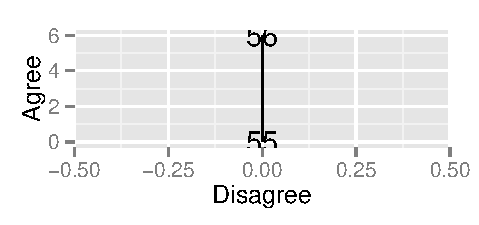
\includegraphics[width=\maxwidth]{figure/unnamed-chunk-31} 

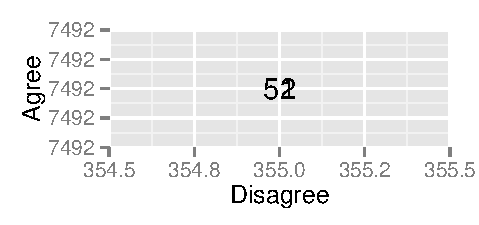
\includegraphics[width=\maxwidth]{figure/unnamed-chunk-32} 

\end{knitrout}

\caption{ROC for Gen1Housemates (left) and Gen2Siblings (right)}
\end{figure}

% latex table generated in R 2.15.3 by xtable 1.7-1 package
% Sun Mar 17 21:48:39 2013
\begin{table}[ht]
\centering
{\large
\begin{tabular}{lrrrrr}
  \hline
R & Implicit2004 & Implicit & Roster & Explicit & Eventual \\ 
  \hline
0 & - &   1 & 478 &  35 & - \\ 
  0.125 &  76 & - &  96 & - &  96 \\ 
  0.130999997258186 & - & - & - &   1 &   1 \\ 
  0.25 &  43 & - & - & 261 & 254 \\ 
  0.375 & 310 & - & - &  54 & - \\ 
  0.5 & 1877 &   6 & - & 3588 & 3565 \\ 
  0.75 &  32 & - & - & - & - \\ 
  1 & - & - & - & - &  11 \\ 
  - & 2964 & 5295 & 4728 & 1363 & 1375 \\ 
   \hline
\end{tabular}
}
\caption{Counts for Gen1Housemates} 
\end{table}
% latex table generated in R 2.15.3 by xtable 1.7-1 package
% Sun Mar 17 21:48:39 2013
\begin{table}[ht]
\centering
{\large
\begin{tabular}{lrrrrr}
  \hline
R & Implicit2004 & Implicit & Roster & Explicit & Eventual \\ 
  \hline
0 & - & - & 478 &  35 & - \\ 
  0.125 &  76 & - &  96 & - &  96 \\ 
  0.130999997258186 & - & - & - &   1 &   1 \\ 
  0.25 &  43 & - & - & 261 & 254 \\ 
  0.375 & 310 & - & - &  54 & - \\ 
  0.5 & 1877 & - & - & 3588 & 3565 \\ 
  0.75 &  32 & - & - & - & - \\ 
  1 & - & - & - & - &  11 \\ 
  - & 2964 & 5302 & 4728 & 1363 & 1375 \\ 
   \hline
\end{tabular}
}
\caption{Counts for Gen1Housemates (Previous version of links)} 
\end{table}
% latex table generated in R 2.15.3 by xtable 1.7-1 package
% Sun Mar 17 21:48:39 2013
\begin{table}[ht]
\centering
{\large
\begin{tabular}{lrrrr}
  \hline
R & Implicit2004 & Implicit & Explicit & Eventual \\ 
  \hline
0.25 & 2221 & 3012 & 2975 & 3442 \\ 
  0.375 & 2663 & - & 244 & 610 \\ 
  0.5 & 5778 & 6731 & 5599 & 6997 \\ 
  0.75 & - &  12 & - &  12 \\ 
  1 &  36 &  27 &  22 &  27 \\ 
  - & 390 & 1306 & 2248 &   0 \\ 
   \hline
\end{tabular}
}
\caption{Counts for Gen2Siblings} 
\end{table}
% latex table generated in R 2.15.3 by xtable 1.7-1 package
% Sun Mar 17 21:48:39 2013
\begin{table}[ht]
\centering
{\large
\begin{tabular}{lrrrr}
  \hline
R & Implicit2004 & Implicit & Explicit & Eventual \\ 
  \hline
0.25 & 2221 & 3012 & 2975 & 3442 \\ 
  0.375 & 2663 & - & 244 & 610 \\ 
  0.5 & 5778 & 6731 & 5599 & 6997 \\ 
  0.75 & - &  12 & - &  12 \\ 
  1 &  36 &  27 &  22 &  27 \\ 
  - & 390 & 1306 & 2248 &   0 \\ 
   \hline
\end{tabular}
}
\caption{Counts for Gen2Siblings (Previous version of links)} 
\end{table}



% latex table generated in R 2.15.3 by xtable 1.7-1 package
% Sun Mar 17 21:48:40 2013
\begin{table}[ht]
\centering
\begin{tabular}{rrrrrr}
  \hline
Count & RImplicit2004 & RImplicit & RExplicit & RRoster & Delta \\ 
  \rowcolor{sosoColor}  \hline
1793 & - & - & 0.500 & - & -4 \\ 
   \rowcolor{sosoColor} 1507 & 0.500 & - & 0.500 & - & -2 \\ 
   \rowcolor{nullColor} 509 & - & - & - & - & 0 \\ 
   \rowcolor{nullColor} 326 & - & - & - & 0.000 & -1 \\ 
   \rowcolor{nullColor} 232 & 0.500 & - & - & - & 0 \\ 
   \rowcolor{sosoColor} 220 & 0.375 & - & 0.500 & - & 0 \\ 
   \rowcolor{sosoColor} 215 & - & - & 0.250 & - & 0 \\ 
   \rowcolor{nullColor} 103 & 0.500 & - & - & 0.000 & 0 \\ 
   \rowcolor{nullColor} 50 & 0.125 & - & - & 0.125 & 0 \\ 
   \rowcolor{nullColor} 48 & 0.375 & - & - & - & 0 \\ 
   \rowcolor{sosoColor} 39 & - & - & 0.375 & - & 0 \\ 
   \rowcolor{nullColor} 34 & - & - & - & 0.125 & 0 \\ 
   \rowcolor{sosoColor} 26 & - & - & 0.000 & - & 0 \\ 
   \rowcolor{sosoColor} 20 & 0.250 & - & 0.500 & - & 0 \\ 
   \rowcolor{sosoColor} 19 & 0.750 & - & 0.500 & - & 0 \\ 
   \rowcolor{sosoColor} 18 & 0.375 & - & 0.250 & - & 0 \\ 
   \rowcolor{sosoColor} 18 & 0.500 & - & 0.250 & - & 0 \\ 
   \rowcolor{sosoColor} 14 & 0.125 & - & 0.500 & - & 0 \\ 
   \rowcolor{nullColor} 13 & 0.375 & - & - & 0.000 & 0 \\ 
   \rowcolor{nullColor} 11 & 0.250 & - & - & 0.000 & 0 \\ 
   \rowcolor{sosoColor} 10 & 0.500 & - & 0.375 & - & 0 \\ 
   \rowcolor{nullColor} 9 & 0.250 & - & - & - & 0 \\ 
   \rowcolor{nullColor} 8 & 0.750 & - & - & - & 0 \\ 
   \rowcolor{sosoColor} 6 & - & - & 0.250 & 0.000 & 0 \\ 
   \rowcolor{sosoColor} 5 & 0.375 & - & 0.375 & - & 0 \\ 
   \rowcolor{nullColor} 5 & 0.750 & - & - & 0.000 & 0 \\ 
   \rowcolor{sosoColor} 5 & - & - & 0.500 & 0.000 & 0 \\ 
   \rowcolor{nullColor} 4 & 0.125 & - & - & - & 0 \\ 
   \rowcolor{nullColor} 4 & 0.375 & - & - & 0.125 & 0 \\ 
   \rowcolor{goodColor} 4 & - & 0.500 & 0.500 & - & 4 \\ 
   \rowcolor{sosoColor} 3 & 0.125 & - & 0.000 & - & 0 \\ 
   \rowcolor{nullColor} 3 & 0.125 & - & - & 0.000 & 0 \\ 
   \rowcolor{sosoColor} 2 & 0.250 & - & 0.250 & - & 0 \\ 
   \rowcolor{nullColor} 2 & 0.500 & - & - & 0.125 & 0 \\ 
   \rowcolor{sosoColor} 2 & - & - & 0.000 & 0.000 & 0 \\ 
   \rowcolor{sosoColor} 2 & - & - & 0.000 & 0.125 & 0 \\ 
   \rowcolor{goodColor} 2 & 0.500 & 0.500 & 0.500 & - & 2 \\ 
   \rowcolor{sosoColor} 1 & 0.125 & - & 0.250 & - & 0 \\ 
   \rowcolor{sosoColor} 1 & 0.125 & - & 0.500 & 0.125 & 0 \\ 
   \rowcolor{nullColor} 1 & 0.250 & - & - & 0.125 & 0 \\ 
   \rowcolor{sosoColor} 1 & 0.375 & - & 0.000 & 0.000 & 0 \\ 
   \rowcolor{sosoColor} 1 & 0.375 & - & 0.500 & 0.000 & 0 \\ 
   \rowcolor{sosoColor} 1 & 0.500 & - & 0.000 & - & 0 \\ 
   \rowcolor{sosoColor} 1 & 0.500 & - & 0.131 & - & 0 \\ 
   \rowcolor{sosoColor} 1 & 0.500 & - & 0.500 & 0.000 & 0 \\ 
   \rowcolor{sosoColor} 1 & - & - & 0.250 & 0.125 & 0 \\ 
   \rowcolor{sosoColor} 1 & - & - & 0.500 & 0.125 & 0 \\ 
  1 & - & 0.000 & - & 0.000 & 1 \\ 
   \hline
\end{tabular}
\caption{Counts for Gen1Housemates} 
\end{table}
% latex table generated in R 2.15.3 by xtable 1.7-1 package
% Sun Mar 17 21:48:40 2013
\begin{table}[ht]
\centering
\begin{tabular}{rrrrrr}
  \hline
Count & RImplicit2004 & RImplicit & RExplicit & RRoster & Delta \\ 
  \rowcolor{goodColor}  \hline
4406 & 0.500 & 0.500 & 0.500 & - & 0 \\ 
   \rowcolor{goodColor} 1599 & 0.250 & 0.250 & 0.250 & - & 0 \\ 
  1095 & 0.500 & 0.500 & - & - & 0 \\ 
   \rowcolor{goodColor} 534 & 0.375 & 0.500 & 0.500 & - & 0 \\ 
   \rowcolor{goodColor} 532 & 0.375 & 0.250 & 0.250 & - & 0 \\ 
   \rowcolor{nullColor} 478 & 0.375 & - & - & - & 0 \\ 
   \rowcolor{sosoColor} 369 & 0.375 & - & 0.250 & - & 0 \\ 
   \rowcolor{sosoColor} 257 & 0.375 & - & 0.500 & - & 0 \\ 
  208 & 0.250 & 0.250 & - & - & 0 \\ 
  169 & 0.375 & 0.500 & - & - & 0 \\ 
  121 & 0.375 & 0.250 & - & - & 0 \\ 
   \rowcolor{goodColor} 119 & - & 0.500 & 0.500 & - & 0 \\ 
   \rowcolor{goodColor} 109 & 0.500 & 0.250 & 0.250 & - & 0 \\ 
   \rowcolor{goodColor} 98 & - & 0.250 & 0.250 & - & 0 \\ 
  91 & 0.250 & 0.250 & 0.375 & - & 0 \\ 
   \rowcolor{badColor} 86 & 0.250 & 0.250 & 0.500 & - & 0 \\ 
   \rowcolor{badColor} 77 & 0.375 & 0.250 & 0.500 & - & 0 \\ 
   \rowcolor{badColor} 75 & 0.500 & 0.500 & 0.250 & - & 0 \\ 
  75 & - & 0.500 & - & - & 0 \\ 
   \rowcolor{goodColor} 73 & 0.250 & 0.500 & 0.500 & - & 0 \\ 
   \rowcolor{sosoColor} 66 & 0.250 & - & 0.250 & - & 0 \\ 
   \rowcolor{badColor} 50 & 0.375 & 0.500 & 0.250 & - & 0 \\ 
   \rowcolor{badColor} 41 & 0.250 & 0.500 & 0.250 & - & 0 \\ 
  41 & 0.500 & 0.500 & 0.375 & - & 0 \\ 
   \rowcolor{sosoColor} 30 & 0.375 & - & 0.375 & - & 0 \\ 
   \rowcolor{sosoColor} 29 & - & - & 0.250 & - & 0 \\ 
   \rowcolor{nullColor} 29 & - & - & - & - & 0 \\ 
  23 & 0.375 & 0.250 & 0.375 & - & 0 \\ 
  23 & 0.375 & 0.500 & 0.375 & - & 0 \\ 
   \rowcolor{goodColor} 21 & 1.000 & 1.000 & 1.000 & - & 0 \\ 
   \rowcolor{badColor} 18 & 0.500 & 0.250 & 0.500 & - & 0 \\ 
   \rowcolor{sosoColor} 17 & 0.250 & - & 0.500 & - & 0 \\ 
  17 & - & 0.250 & - & - & 0 \\ 
  15 & 0.500 & 0.250 & 0.375 & - & 0 \\ 
   \rowcolor{nullColor} 14 & 0.250 & - & - & - & 0 \\ 
  13 & 0.250 & 0.500 & - & - & 0 \\ 
  12 & 1.000 & 0.750 & - & - & 0 \\ 
  11 & 0.500 & 0.250 & - & - & 0 \\ 
  10 & 0.250 & 0.500 & 0.375 & - & 0 \\ 
   \rowcolor{sosoColor} 6 & - & - & 0.500 & - & 0 \\ 
   \rowcolor{badColor} 4 & - & 0.250 & 0.500 & - & 0 \\ 
   \rowcolor{badColor} 4 & - & 0.500 & 0.250 & - & 0 \\ 
   \rowcolor{sosoColor} 3 & 0.250 & - & 0.375 & - & 0 \\ 
   \rowcolor{sosoColor} 3 & 0.500 & - & 0.250 & - & 0 \\ 
  3 & 1.000 & 1.000 & - & - & 0 \\ 
  3 & - & 0.250 & 0.375 & - & 0 \\ 
  3 & - & 0.500 & 0.375 & - & 0 \\ 
   \rowcolor{sosoColor} 2 & 0.500 & - & 0.500 & - & 0 \\ 
   \rowcolor{sosoColor} 2 & - & - & 0.375 & - & 0 \\ 
   \rowcolor{goodColor} 1 & 0.500 & 1.000 & 1.000 & - & 0 \\ 
  1 & 0.500 & 1.000 & - & - & 0 \\ 
   \rowcolor{nullColor} 1 & 0.500 & - & - & - & 0 \\ 
  1 & - & 1.000 & - & - & 0 \\ 
   \hline
\end{tabular}
\caption{Counts for Gen2Siblings} 
\end{table}



\end{document}
